\documentclass{standalone}
\usepackage{tikz,color}
\begin{document}

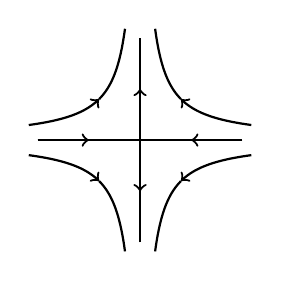
\begin{tikzpicture}[scale=1.3]
\draw [->,thick] (-1,0) to (-0.5,0);
\draw [->,thick] (1,0)  to (0.5,0);
\draw [-,thick ] (-1,0) to (1,0);
\draw [->,thick] (0,0) to (0,-0.5);
\draw [->,thick] (0,0)  to (0,0.5);
\draw [-,thick ] (0,-1) to (0,1);
\draw [-,thick, domain=-1:0, samples=25] plot({0.4*exp(\x)},{0.4*exp(-\x)});
\draw [<-,thick, domain=  0:1, samples=25] plot({0.4*exp(\x)},{0.4*exp(-\x)});
\draw [-,thick, domain=-1:0, samples=25] plot({-0.4*exp(\x)},{0.4*exp(-\x)});
\draw [<-,thick, domain=  0:1, samples=25] plot({-0.4*exp(\x)},{0.4*exp(-\x)});
\draw [-,thick, domain=-1:0, samples=25] plot({0.4*exp(\x)},{-0.4*exp(-\x)});
\draw [<-,thick, domain=  0:1, samples=25] plot({0.4*exp(\x)},{-0.4*exp(-\x)});
\draw [-,thick, domain=-1:0, samples=25] plot({-0.4*exp(\x)},{-0.4*exp(-\x)});
\draw [<-,thick, domain=  0:1, samples=25] plot({-0.4*exp(\x)},{-0.4*exp(-\x)});

\end{tikzpicture}
\end{document}
